% 文档类
\documentclass[13pt]{ctexart}
% 设置页面
\usepackage{geometry}
% 插图片
\usepackage{graphicx}
% 设置标题 重命名为英文
\renewcommand{\figurename}{Figure}
\renewcommand{\tablename}{Table}
\renewcommand{\contentsname}{Contents}
% 设置摘要页缩减 
\usepackage{changepage}
% 便于修改字体
\usepackage{fontspec}
% 设置页眉页脚
\usepackage{fancyhdr}
% 清空页眉页脚
\pagestyle{fancy}
% 设置列表缩进
\usepackage[shortlabels]{enumitem}
% 设置修改默认的section标题大小
\usepackage{titlesec}
\titleformat*{\section}{\LARGE}
\titleformat*{\subsection}{\Large}
\titleformat*{\subsubsection}{\Large}
% 使用数学宏包
\usepackage{amsmath}
% 设置表格的列格式
\usepackage{array}
% 三线表宏包
\usepackage{booktabs}
% 设置产考文献不输出默认名
\usepackage{etoolbox}
\patchcmd{\thebibliography}{\section*{\refname}}{}{}{}
% 引入网站作为参考文献
\usepackage{url}
% 设置等宽的代码字体
\setmonofont{Courier New}
% 颜色
\usepackage{xcolor}
% 代码高亮方案宏包
\usepackage{listings}
\definecolor{CPPLight}  {HTML} {686868}
\definecolor{CPPSteel}  {HTML} {888888}
\definecolor{CPPDark}   {HTML} {262626}
\definecolor{CPPBlue}   {HTML} {4172A3}
\definecolor{CPPGreen}  {HTML} {487818}
\definecolor{CPPBrown}  {HTML} {A07040}
\definecolor{CPPRed}    {HTML} {AD4D3A}
\definecolor{CPPViolet} {HTML} {7040A0}
\definecolor{CPPGray}  {HTML} {B8B8B8}
\lstset{
	basicstyle=\ttfamily,
	breaklines=true,
	framextopmargin=50pt,
	frame=bottomline,
	columns=fixed,       
    %numbers=left,                                       % 在左侧显示行号
	frame=none,                                          % 不显示背景边框
	backgroundcolor=\color[RGB]{255,255,255},            % 设定背景颜色
	keywordstyle=\color[RGB]{40,40,255},                 % 设定关键字颜色
	numberstyle=\footnotesize\color{darkgray},           % 设定行号格式
	commentstyle=\itshape\color[RGB]{0,96,96},                % 设置代码注释的格式
	stringstyle=\slshape\color[RGB]{128,0,0},   % 设置字符串格式
	showstringspaces=false,                              % 不显示字符串中的空格
	language=python,                                     % 设置语言
	morekeywords={alignas,continute,friend,register,true,alignof,decltype,goto,
		reinterpret_cast,try,asm,defult,if,return,typedef,auto,delete,inline,short,
		typeid,bool,do,int,signed,typename,break,double,long,sizeof,union,case,
		dynamic_cast,mutable,static,unsigned,catch,else,namespace,static_assert,using,
		char,enum,new,static_cast,virtual,char16_t,char32_t,explict,noexcept,struct,
		void,export,nullptr,switch,volatile,class,extern,operator,template,wchar_t,
		const,false,private,this,while,constexpr,float,protected,thread_local,
		const_cast,for,public,throw,std},
	emph={map,set,multimap,multiset,unordered_map,unordered_set,numpy,graph,path,append,extend,
		unordered_multiset,unordered_multimap,vector,string,list,deque,
		array,stack,forwared_list,iostream,memory,shared_ptr,unique_ptr,
		random,bitset,ostream,istream,cout,cin,endl,move,default_random_engine,
		uniform_int_distribution,iterator,algorithm,functional,bing,numeric,},
	emphstyle=\color{CPPViolet}, 
}

\begin{document}
\newgeometry{top = 1cm, right = 2.54cm, left = 2.54cm, bottom = 2.54cm}
% 第一页的字体为times new roman
\setmainfont{Times New Roman}
\thispagestyle{empty}

\begin{table}[h]
    \quad { }  \begin{minipage}[t]{5.5cm}
        % arraystretch 是调节列高
        \begin{tabular}[t]{>{\centering\arraybackslash}b{10em}}
            \fontsize{12pt}{10pt}\selectfont \textbf{Problem Chosen}\\ [2pt]
            {\color{red} \fontsize{20pt}{10pt}\selectfont ABCDEF}
        \end{tabular}
    \end{minipage}
    \begin{minipage}[t]{5.2cm}
        \begin{tabular}[t]{>{\centering\arraybackslash}p{10em}}
            \fontsize{12pt}{10pt}\selectfont \textbf{2020} \\ [-2pt]
            \fontsize{12pt}{10pt}\selectfont \textbf{MCM/ICM} \\ [-2pt]
            \fontsize{12pt}{10pt}\selectfont \textbf{Summary Sheet}
        \end{tabular}
    \end{minipage}
    \begin{minipage}[t]{3cm}
        \begin{tabular}[t]{>{\centering\arraybackslash}b{12em}}
            \fontsize{12pt}{10pt}\selectfont \textbf{Team Control Number} \\ [2pt]
            {\color{red} \fontsize{21pt}{10pt}\selectfont 1111111}
        \end{tabular}
    \end{minipage}
\end{table}
\vspace{-20pt}
\noindent{\rule{\textwidth}{0.5mm}}

% 标题
{\centering\fontsize{18}{16}\selectfont\textbf{{Analysis and Supression of Opioid Spread}}
% 摘要
\vspace{10pt} 

\fontsize{13}{10}\selectfont\textbf{{Summary}}\par}

\vspace{10pt}

% 正文字体 13 pt
\fontsize{13}{12.5}\selectfont

\begin{adjustwidth}{1cm}{1cm}
\indent { }{ }{ }{ }{ }{ }We propose a model to describe the characteristics of the number, rate and direction of opioid spread in and between states and counties using transition matrices. The result shows that among the five given states, Ohio is most likely the source of opioid cases and has frequent opioid transition with Pennsylvania and Kentucky. We also find that if no effective regulatory measures are imposed, the number of drug cases in Ohio will increase up to 141,266 in the next decade. The spread of opioids between counties was analyzed in the same way, and the result is shown in Figure 3.

We determine two epidemic thresholds based on characteristics of opioid spread, with respect to the number of opioid cases and opioid spread rate respectively. We perform simulations to forecast the number of opioid cases in states and counties. The result shows that the number of narcotic analgesics cases in Ohio reaches the threshold in 2022, and the number of heroin cases in Pennsylvania reached the threshold in 2023.

We analyze the correlations between the number of opioid cases and various socio-economic factors using information entropy. We find that the number of opioids cases demonstrates high correlations with disability status, educational level, family status and adolescents. Therefore, we provide suggestions based on these factors to help suppress opioid spread. We also evaluate the effectiveness of these strategies on both the spread rate and the number of opioid cases. The result shows that when the amount of opioids spread is reduced to 74.5\%, the amount of opioids will stay on a relatively low level, and become lower than that of 2010 after 5 years.

We also do sensitivity analysis of various parameters to prove the robustness of our model. The result shows that both the continuous and periodical inflows lead to increase in the number of opioids in the state, and the increased amount depends on the specific transition amount.

\vspace{15pt}
\textbf{key words} : Transition matrix; Multi-level thresholds; Information entropy
\end{adjustwidth} 

% 开始写 memo 信
% 更换字体为 palatino 也可以不换
\setmainfont{TeX Gyre Pagella}
\newpage
\newgeometry{left = 3.5cm, right = 3.5cm}
\thispagestyle{empty}

{\centering \fontsize{18pt}{14pt}\selectfont \textbf{MEMO}\par}

\noindent FROM: Team {} 1917694 , MCM C

\noindent To: The group of Governors

\noindent Date: January 28, 2019

\vspace{10pt}

Dear Officials:

It is our honor to help you with analyzing the spread and characteristics of opioid. We are writing this letter to report our findings.

We analyzed the characteristics of opioid spread in the five states and counties, and found that if left uncontrolled, the opioid abuse will continue to spread, and the number of drug users will increase. We also found that there is no obvious relationship between the spread of opioid use and the geographical location. We deduced that Ohio is most likely the originated state of opioid use, and the drug cases will increase significantly over time. Of all five states, West Virginia shows a relatively healthy status. We also analyzed each county in the five states. Taking West Virginia as an example, Monongalia and Berkeley may be the originating counties for heroin transmission, and drug cases in these two counties are mainly spread to Kanawha and Berkeley.

We determined two epidemic thresholds based on characteristics of opioid spread, with respect to the number of opioid cases and opioid spread rate respectively. We found that the number of narcotic analgesics cases in Ohio reaches the threshold in 2022, and the number of heroin cases in Pennsylvania reached the threshold in 2023.

We analyzed the correlations between the number of opioid cases and various socio-economic factors. We found that the number of opioids cases shows high correlations with disability status, educational level, family status and adolescents. Therefore, we provide suggestions based on these factors to help suppress opioid spread. We also evaluate the effectiveness of these strategies. The result shows that when the amount of drug spread is less than 26.3\% on before, the number of drug users will be significantly reduced in 3 years, and become lower than that of 2010 in 5 years. 

We also do sensitivity analysis of our model. We found that inflows of drugs from outside the states also plays an important role in affecting the number of opioid cases.

Based on our analysis, we provide some suggestions to effectively prevent opioid spread:

1. National and local governments play an important role in detecting and preventing opioid overdose and abuse. Monitoring systems and early warning mechanisms should be established to effectively detect and respond to the spread of opioid abuse.

2. Provide more job opportunities to alleviate people's pressure, even to set up a free subsidy program. The local government should also publicize the harm of opioids abuse.

3. Prescriptions and sales of opioids should be strictly controlled, and a feedback mechanism for mandatory postoperative hospital visits should be established. The patients should also be examined for abuse of opioids during the hospital examination.

4. Impose careful check and strict management of logistics, to reduce the impact of opioids from outside the states.

We believe that our model is useful for preventing opioid spread in the future. You are welcome to contact us at any time for further cooperation.

% 信多出一页,清理页眉页脚
\thispagestyle{empty}
% 信的结尾
{\raggedleft
Sincerely yours

MCM C Team 1917694\par
}

% 目录页
\newpage
\thispagestyle{empty}
\tableofcontents
\newpage
% 目录页后面是第一页
\setcounter{page}{1}

% 开始写正文
% 设置正文的页边距
\newgeometry{top=3cm, left=3.5cm, right=3.5cm}
% 设置正文的页眉页脚
\fancyhf{}
\fancyhead[C]{ }
% 此处修改右上角页码
\fancyhead[R]{Page \thepage\ of 18}
%\fancyhead[R]{Page \thepage\ of 15}
\fancyhead[L]{Team \# 1917694}
\fancyfoot[C]{\bfseries\thepage}
\textbf{\section{Introduction}}
\textbf{\subsection{Restatement of the Problem}}
Many people nowadays rely heavily on opioids and even die from opioid overdose. Reducing opioid use and suppressing opioid spread becomes an urgent task. Therefore we are facing the following problems:

\begin{itemize}
	\item Describe the spread and characteristics of opioids in and between the given states and counties, analyze the characteristics of opioid spread, and find the source of opioid use cases.
	\item If opioid cases continue to spread, determine the epidemic threshold for the government to take action and analyze where and when they will occur.
	\item Analyze the correlation between the number of opioid cases and the socio-economic factors, then modify the model to include important factors.
	\item Establish effective policies to prevent the spread of opioids and evaluate the effectiveness of policies.
\end{itemize}
\textbf{\subsection{Our Works}}

\begin{itemize}
	\item First, we build a model to analyze the characteristics of opioid spread, and determine the source of opioid cases based on the characteristics.
	\item Then, we determine two thresholds with respect to the spread rate and the number of opioid cases, perform simulations to evolve the opioid spread process to determine where and when the government should take actions first.
	\item We use information entropy to measure the correlations between the number of opioid cases and the socio-economic factors, and propose reasonable suggestions for those factors with high correlation with the number of opioid cases.
	\item Finally, we establish effective policies and perform simulations to evolve the spread of opioids, analyze the result to determine when opioid spread can be successfully suppressed, and quantify the goals that government needs to achieve.
\end{itemize}
\textbf{\section{Assumptions and Notations}}
\vspace*{-10pt}
\textbf{\subsection{Assumptions}}
Due to the lack of necessary data, we make the following assumptions to help us perform modeling.
\begin{itemize}[itemsep=0.3ex, leftmargin=1.2cm]
	\item[1.] Inflow of drugs from outside of the five states are neglected.
	\item[2.] The microscopic behaviors of opioid transmission are ignored.
\end{itemize}
\textbf{\subsection{Notations}}
Here are all the notations and their meanings in this paper.
\begin{table}[h]
	\centering
	\vspace{3pt}
	\begin{tabular}{>{\centering\arraybackslash}p{5em}>{\centering\arraybackslash}p{30em}}
	\toprule % 绘制第一条线
	Symbol & Meaning \\ \midrule
	$t$ & Time \\
	$N$ & Total reported opioid cases\\
	$N_t$ & Total reported drug cases\\
	$\lambda$ & Average cases induced by a single case\\
	$A_t$ & Status at $t$ \\ 
	$E$ & Set containing socio-economic factors with high correlation $t$ \\
	$T$ & Transition matrix\\ 
	$i(t)$ & Proportion of opioid cases in all drug cases at $t$ \\
	$\mu_1$ & Average number of drug cases induced by an existing drug case \\
	$\mu_2$ & Number of opioid cases induced among all drug cases \\
	$\gamma$ & Drug spread slow down factor \\
	$i_0$ & Status at $t$ \\ 
	$H$ & Information Entropy \\ 
	$p_0$ & Initial number of drug cases\\
	\bottomrule
	\end{tabular}
\end{table}

\textbf{\section{Model Construction}}
Census data will have certain deviations. We don't consider statistical errors of the provided census data and just use the values provided.
\textbf{\subsection{Opioid Spread Model}}
As is well known, spreading of illegal drugs are elusive, therefore we do not consider the ways, actions and tools of spreading opioid uses. Instead we focus on analyzing the characteristics of drug use spreading, including the amount of transfer, rate of change and location, in order to obtain conclusions that are convenient for the administration and control of government departments.

According to the report on opioid use published by NFLIS\cite{characteristic}, we define the drug spread characteristics as the number of cases, the rate of change, and the location of use:

\begin{itemize}
	\item Distribution of drug cases: Indicates the number of drug cases over time in a region.
	\item Rate of change: Describes the growth rate of the number of drug cases over time (a positive growth rate indicates a normal trend in drug spread, while a negative growth rate indicates a downtrend).
	\item Location of drug use: Indicates regions where drug cases are mainly concentrated and regions where drug cases are reported.
\end{itemize}

\textbf{Distribution of drug cases}\quad A state can be transferred to a next state by applying a transition matrix \cite{pagerank},therefore we construct a transition matrix $T$, an element $T_{ij}$ in $T$ indicates the proportion of drug cases flowing from region $i$ to region j $i$ to the total drug cases in region $i$. We define a matrix $A_{2010}$ as the drug cases reported in 2010, and similarly $A_{2011}$ as the drug cases reported in 2011. Then under the influence of $T$, $A_{2010}$ transfers to $A_{2011}$. We then derive the general form of drug transmission based on the reasoning above as
\begin{equation}
	T \cdot A_{t-1}=A_t \implies T=A_t \cdot A_{t-1}^{+}
	\label{eq_pagerank}
\end{equation}
After solving the transition matrix $T$, which are different across years, we can obtain information on the spread of drugs.

We define $\beta$ as the average amount of drugs in a single drug case, $T_{ij}$ describes the flow of drugs from region $i$ to region $j$. We define $\eta$ as the proportion of drugs flowing out of region $i$, then an $\eta$ less than 1 indicates there are drugs consumed in region $i$, and an $\eta$ greater than 1 indicates there are drugs flowing in from other regions.

\textbf{Location where specific drug use starts}\quad We first take the mean value of the transition matrices $T$ across all given years to get the average transition matrix $T_{\mathrm{mean}}$ in order to eliminate the the effects of anomalous propagation. Each element in the matrix $T_{\mathrm{mean}}$ describes the flow of drugs, and the location where specific opioid use might have started can be determined based on the largest outflow. Furthermore, without government intervention, under the effect of the transition matrix $T$, the evolution of drug use transmission will eventually show a stable state \cite{page_stable}. Therefore, we compute the drug cases vector $A_{i}$ as time $t$ approaches infinity according to Formula \ref{eq_pagerank}, to determine which regions have high incidences of drug cases, and then take action.

\textbf{Drug transmission rate}\cite{SIR_mu}\quad We define $N_t$ as the number of reports of all drug cases, and the initial number of drug cases is $p_0$. We also define $i(t)$ as the proportion of opioid cases in all drug cases at $t$, and the initial proportion of opioid cases is $i_0$.

We first consider the spread of drug use towards non-drug users. Assuming that the average number of drug cases induced by an existing drug case is $\mu_1$, we establish the following equation:
\begin{equation}
	\frac{\mathrm{d}N_t}{\mathrm{d}t}=N_t\mu_1,N_t(0)=p_0
	\label{S}
\end{equation}
The solution to the above equation is
\begin{equation}
N_t(t)=p_0e^{\mu_1t}
\end{equation}
This indicates that in the absence of any government precautions, the number of drug cases will grow exponentially over time, resulting in severe harm, as shown in Figure \ref{spread_rate}(a).

We then consider the spread of opioids in all drug cases. We define $\mu_2$ as the number of opioid use cases induced by an opioid use case among all drug cases. Therefore, $(1-i(t))\mu_2$ represents the increase in the number of opioid use cases among all drug cases as induced by a single opioid use case. Also notice that the total number of opioid use cases is $N_ti(t)$, thus the total increase in the number of opioid use cases among all drug cases is $N_ti(t)\mu_2(1-i(t))$. Therefore we establish the following equation:
\begin{equation}
	N_t \frac{\mathrm{d}i}{\mathrm{d}t}=
	N_t \mu_2 i(t)(1-i(t)),i(0)=i_0 
	\label{SI}
\end{equation}
The solution to the above equation is
\begin{equation}
i(t)=\frac{1}{1+(\frac{1}{i_0}-1)e^{-t\mu_2}}
\end{equation}
which indicates that $i(t)$ is an S-shaped growth curve, as shown in Figure \ref{spread_rate}(b). The derivative $\mathrm{d}i/\mathrm{d}t$ reaches the maximum at $t=0.5$, at which time the opioid use case grows the fastest, indicating a potential opioid use outbreak.

\begin {figure}[h]
	\centering % 居中显示
	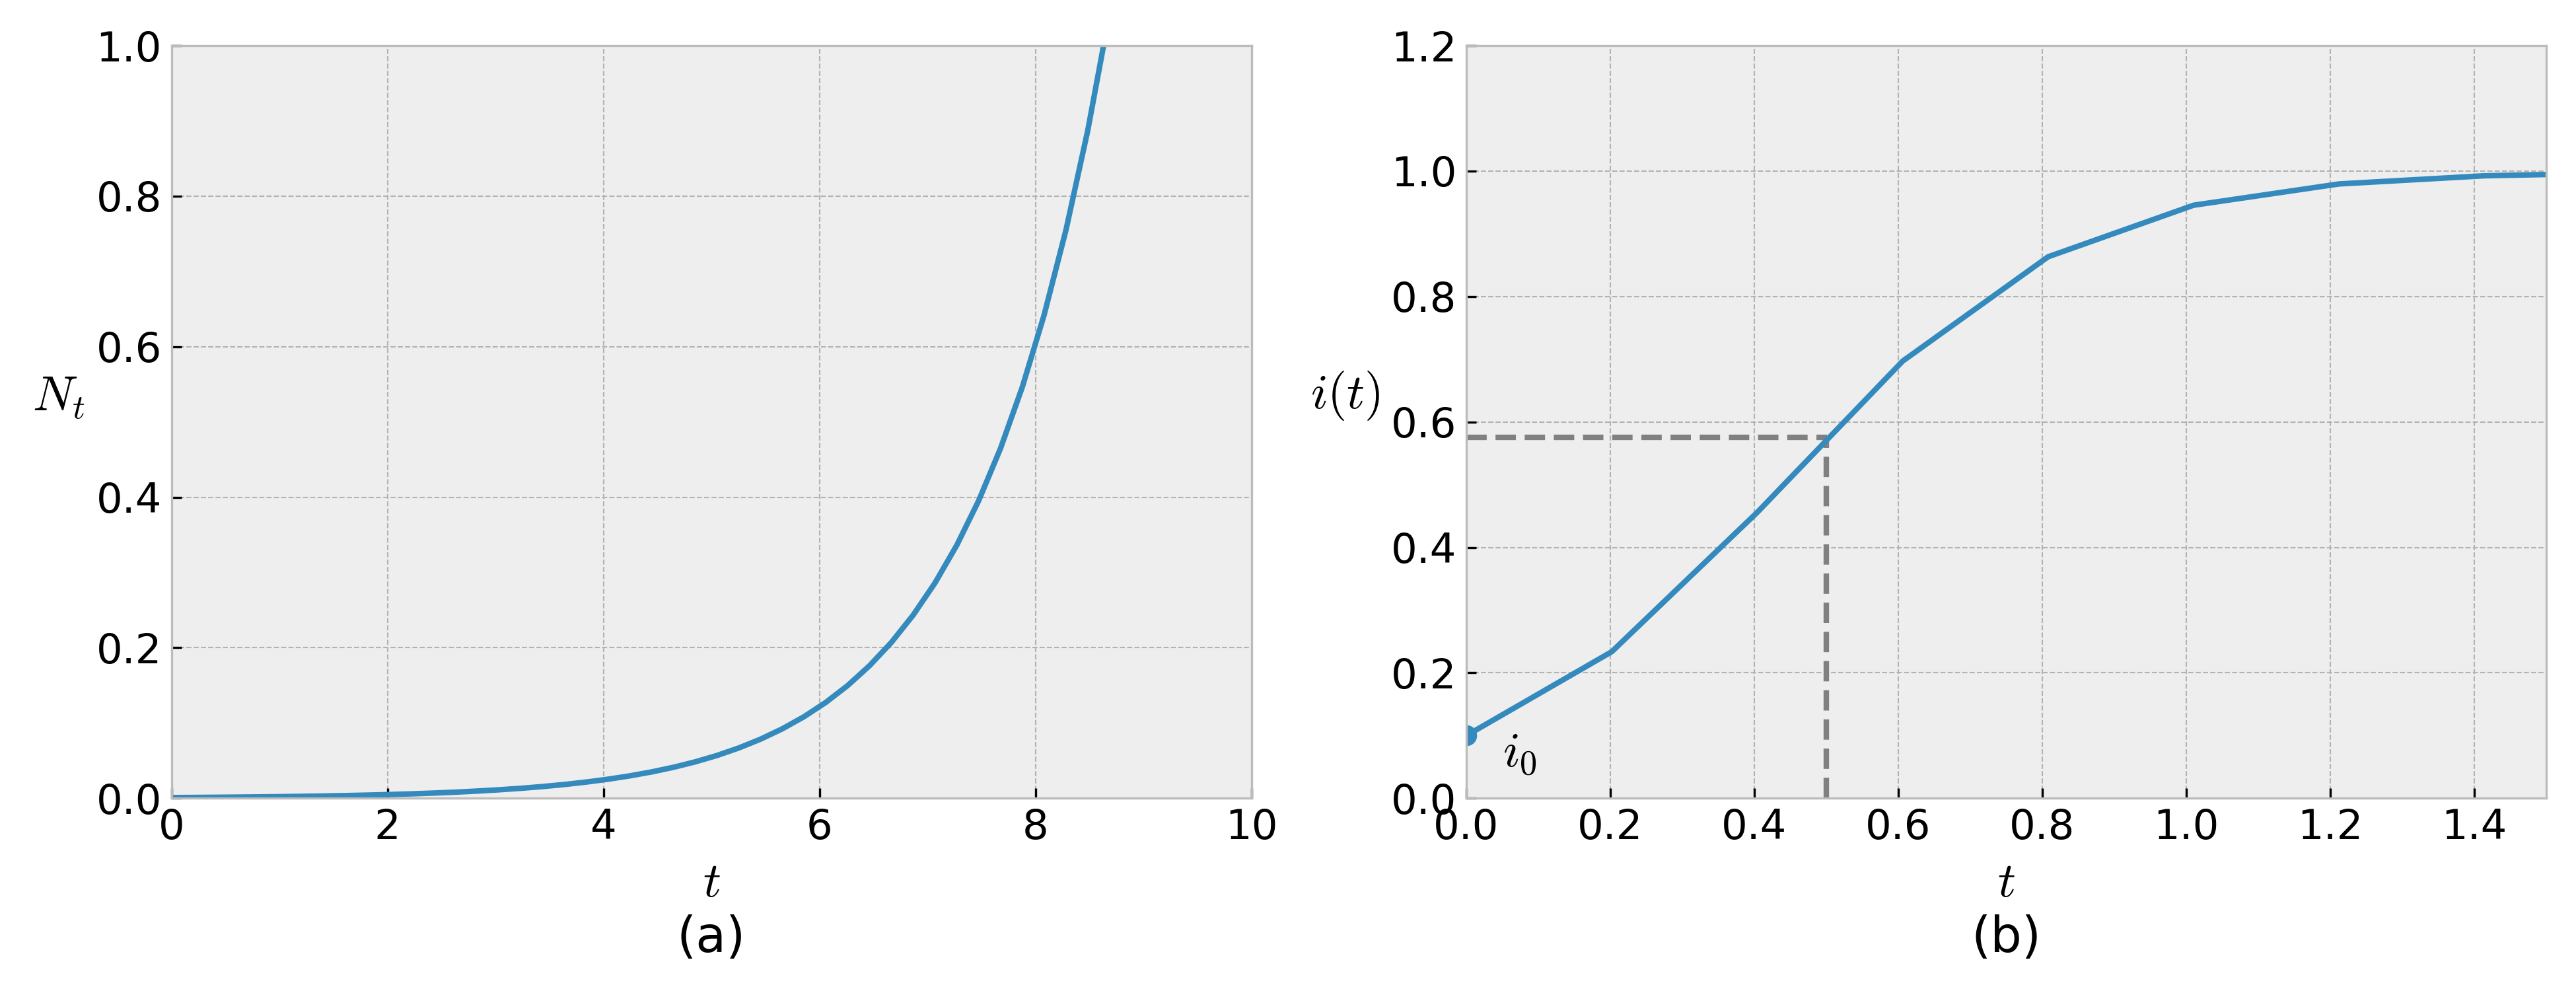
\includegraphics[width=13cm,height=5.5cm]{1.png}
	\caption{Drug cases and proportion of opioid cases over time} % 标题
	\label{spread_rate}
\end {figure}
\textbf{\subsection{Determining the Epidemic Threshold}}
Since the number of drug cases, population and level of economic development are different between states and counties, the epidemic threshold is calculated from a statistical perspective, and each state and county should have different epidemic thresholds. In addition, the excess of the amount and speed of drug transmissions should both raise the government's concern, therefore two epidemic thresholds are set in consideration of both aspect, respectively.

For the epidemic threshold in the number of drug cases, $m+2\sigma$ is generally considered as a gold standard, where $m$ and $\sigma$ denote the mean and standard deviation of the number of drug cases respectively\cite{threshold_who}. The calculated threshold is considered constant over time, because the number of drug cases increases by year, and by setting a relatively low threshold, the government can stay vigilant and therefore suppress the number of drug cases promptly.

For the epidemic threshold in transmission speed, we compute the derivative of $N_t(t)$, which gives us
\begin{equation}
	N_t'(t)=\mu_1p_0e^{\mu_1t}
\end{equation}

We observe that the growth rate $N_t'(t)$ turns out to be an exponential function, and the number of drug cases will keep growing if no interventions are imposed. So we set the initial growth rate at $t=0$ to be the baseline growth rate, which turns out to be $\mu_1p_0$. Here we find that the growth rate threshold is related to $\mu_1$ and $p_0$, where $p_0$ reflects the amount of drug users in a given region, and $\mu_1$ reflects the administrative state such as the strictness of management.

\textbf{\subsection{Modification to the Opioid Spread Model}}
\textbf{\subsubsection{Determining Correlation Using Information Entropy}}
There are uncertainties and randomness in the process of drug transmission, and the way to eliminate uncertainty is to introduce new information from the outside, and using this information can eliminate some of the uncertainties. Information entropy is a common measurement of uncertainty.

For the number of drug cases $N$, its uncertainty $H(N)$ is computed according to the following formula:
\begin{equation}
H(N)=-\sum P(N)\cdot \log_2 P(N)
\end{equation}

Suppose the introduction of information from the socio-economic data provided by the U.S. Census Bureau can reduce uncertainty. The more uncertainties are reduced, the stronger the correlation \cite{entroy}. We introduce an socio-economic factor as a piece of information $Y$, then we calculate the uncertainty of $N$ under the condition of $Y$, i.e. the conditional entropy $H(N|Y)$:

\begin{equation}
H(N|Y)=-\sum P(N,Y)\log_2 P(N|Y)
\end{equation}

The conditional entropy $H(N|Y)$ after the introduction of information $Y$ is less than the information entropy $H(N)$, which indicates that the introduction of the socio-economic factor reduced the uncertainty. We define $\Delta h$ to be the reduction in information:
\begin{equation}
	\Delta h= H(X)-H(X|Y)
	\label{delta}
\end{equation}

There are multiple attributes in the provided data. although it is possible to calculate the conditional entropy $H(N|Y_1, Y_2,...,Y_n)$ under multiple information, it is difficult to determine the optimal order in which the information is integrated, for example, whether $H( N|Y_1, Y_2, Y_4)$ reduces more uncertainty than $H(N|Y_1, Y_2, Y_3)$. Therefore we only calculate $\Delta h$ of the number of drug cases and one other socio-economic factor. After calculating $\Delta h$ for all socio-economic factors, those factors with larger value of $\Delta h$ are kept in a set $E$. The socio-economic factors in the set $E$ demonstrate a strong correlation with the number of drug cases, and we make suggestions to the government based on the phenomena represented by these attributes.
\textbf{\subsubsection{Modifying Our Model with Hidden States}}
As depicted above, the socio-economic factors in the set $E$ demonstrate strong correlations with the number of reported drug cases. Therefore, in order to improve our model's performance, it is necessary to integrate these factors into our opioid spread model.

The specific relationships (e.g. linear or nonlinear) between the number of drug cases and the socio-economic factors are unclear, and there does not yet exist formulae to describe the relationships between them. Although the number of drug cases are provided, there is no effective way to figure out the drug transmission processes. Therefore the numbers of drug cases $A$ is defined as the hidden state, and the observable socio-economic factors $E$ are defined as explicit states. Then we modify our opioid spread model to take both the explicit states and the hidden states into consideration, as illustrated in Figure 2.

\begin {figure}[h]
	\centering % 居中显示
	
\includegraphics[width=13cm,height=4cm]{2.png}
	\caption{Illustration for model structure} % 标题
	\label{hmm}
\end {figure}

In the Figure \ref{hmm}, the transition between hidden states can be calculated by the transition matrix $T$. An explicit state can be seen as a window through which the corresponding hidden state can be observed. The correlation between a hidden state and the corresponding explicit state can be calculated according to  Formula (\ref{delta}).

\textbf{\subsubsection{Analysis of the Modified Model}}

The structure of our improved model shares lots of similarities with the hidden Markov model. Our improved model can solve the following problems \cite{hmm_1}:

Given the information of the socio-economic factor set $E$ in the past few years as the explicit state and the corresponding number of drug cases as the hidden state. Also given the specific explicit state value $D$, then the transition matrix $T_{max}$ which is most likely to produce $D$ can be calculated:

\begin{equation}
	T_\mathrm{max}=\mathrm{ArgMax}\prod_{t=1}^{n}(P(E_t|A_t)|P(T_t|T_{t-1}))
\end{equation}
where $E_t, A_t, T_t$ represents the explicit state, hidden state, and transition matrix at time $t$. The transition matrix $T$ with the highest probability can be obtained based on the distribution of the population, and the result becomes more stable over time. With the transition matrix, which indicates the drug case transmission, the government will be able to effectively monitor and prevent the drug spread in the region, thus reduce the number of drug cases.
\textbf{\section{Model Simulation and Analysis}}
\textbf{\subsection{Describing Characteristics of Opioid Spread}}

Using the provided data, we perform simulation on our model to simulate the drug spread in and between states and counties, then analyze the resulting spread characteristics.

Opioid spread between counties: We take West Virginia as an example to analyze the transmission of synthetic opioid and heroin inside the state. The spread status of heroin is shown in Figure \ref{WV}.

\begin {figure}[h]
	\centering % 居中显示
	
\includegraphics[width=15cm,height=12cm]{3.png}
	\caption{Transition matrix for opioid spread rate in West Virginia} % 标题
	\label{WV}
\end {figure}

We draw a the conclusion that Monongalia (54061) and Berkeley (54003) are most likely to be the originating counties for heroin transmission, and heroin in these two counties are mainly transferred to Kanawha (54039) and Berkeley. In addition, Berkeley has a large flow rate, and as both an inflow and outflow  region of heroin, therefore it is necessary to strengthen supervision on heroin transmission in this region. For other counties such as Cabell (54011), Harrison (54033) and Marion (54049) which have large heroin inflows, it is also necessary to strengthen supervision on drugs and check the logistics.

We analyze the transmission of narcotic analgesics (synthetic opioids) in West Virginia in the same way. We find that Mercer (54055) has a high inflow and outflow of narcotic analgesics. Therefore we can deduce that Mercer may be the manufacturing and main consumption county of analgesics. For other counties such as Raleigh (50481), Nicholas (54067), and Kanawha (54039), there are also large outflows and use cases, which indicates they are also main consumption and spread regions of analgesics in West Virginia. The transmission flows in the remaining counties are significantly lower. The resulting figures are in Appendix A.

Opioid spread between states: We analyze the transmissions of all drugs within the five states, and plot the heat map for the transition matrix of analgesics and heroin. The results are shown in Figure \ref{five}.

\begin {figure}[h]
	\centering % 居中显示
	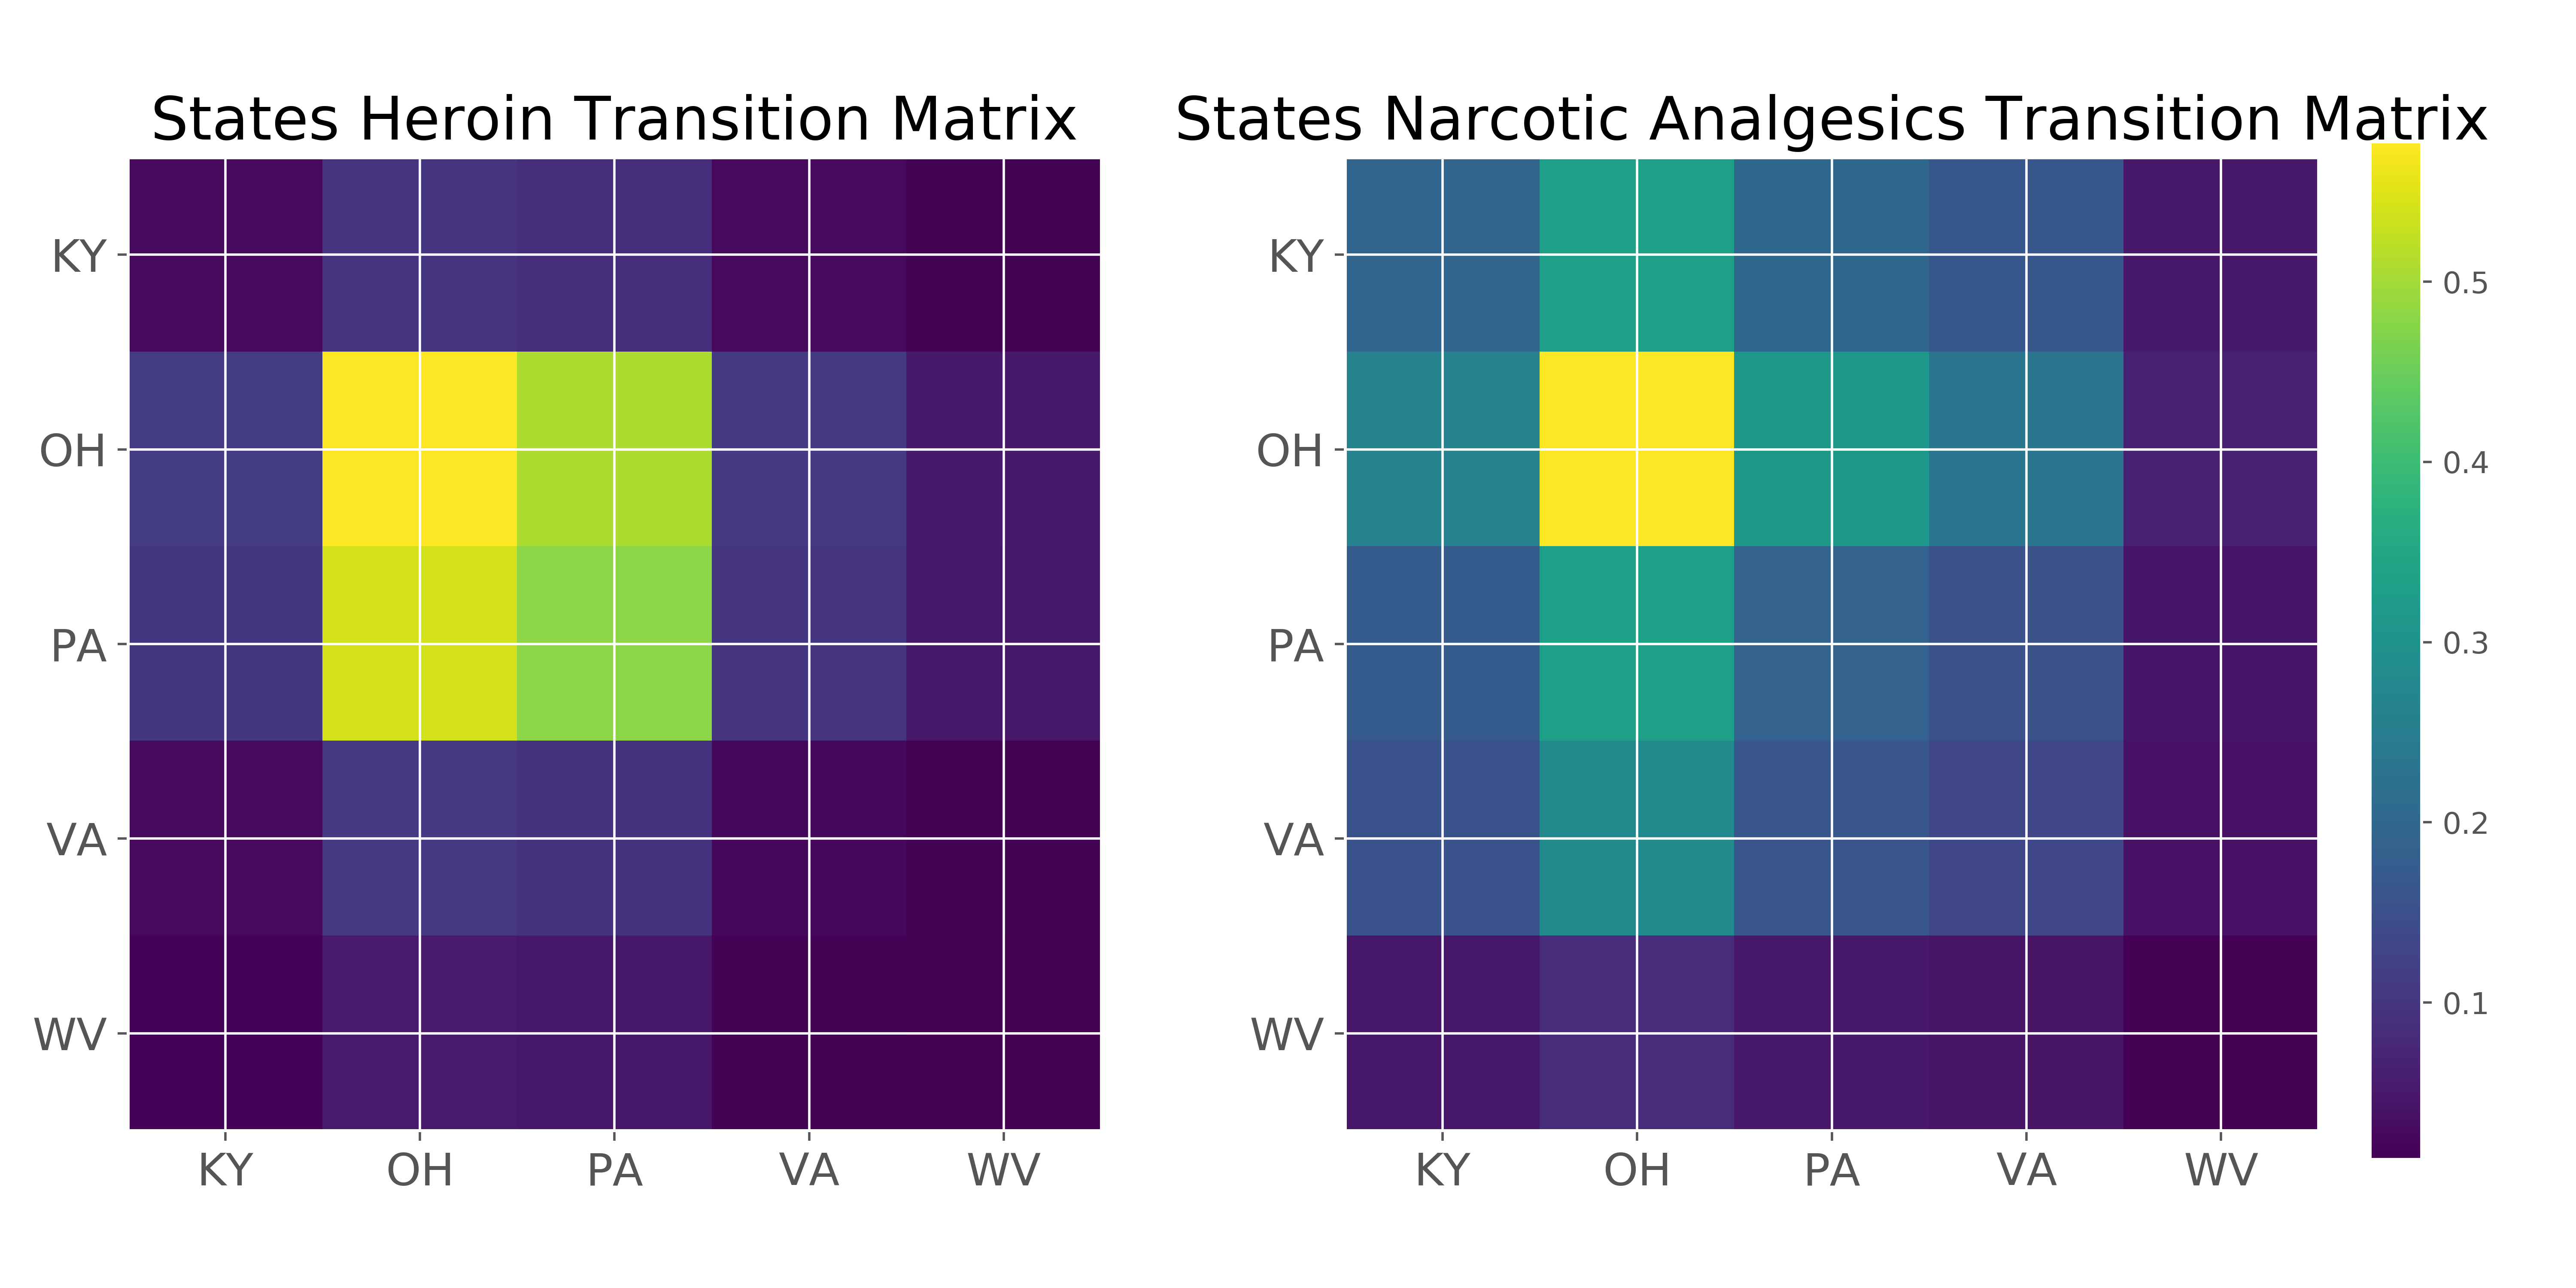
\includegraphics[width=13cm,height=6cm]{4.png}
	\caption{Heat map of transition matrix for five states} % 标题
	\label{five}
\end {figure}

We find that analgesic and heroin transmissions between Kentucky, Ohio, and Pennsylvania are frequent. We also notice that these three states were located at edges relative to other states geographically, indicating that geographical locations generally do not prevent the spread of drugs. In addition, the consumption and outflow of drugs in Ohio are high, thus should raise the government's attention.

Source analysis of drug cases: In order to eliminate the effects of abnormal transmission, we take the average of the transmission matrices in 2010-2017 in each state as the drug transmission matrix. The resulting transition matrix is shown in Table \ref{trans}.

\begin{table}
	\centering
	\caption{Transition matrix for states}
	\begin{tabular}{>{\centering\arraybackslash}p{4em}>{\centering\arraybackslash}p{3em}>{\centering\arraybackslash}p{3em}>{\centering\arraybackslash}p{3em}>{\centering\arraybackslash}p{3em}>{\centering\arraybackslash}p{3em}}
		\toprule
		{State}& KY & OH & PA & VA & WV\\\midrule
		KY & 0.044 & 0.158 & 0.124 & 0.056 & 0.012 \\ 
		OH & 0.146 & 0.539 & 0.405 & 0.184 & 0.037 \\ 
		PA & 0.128 & 0.454 & 0.359 & 0.161 & 0.035 \\ 
		VA & 0.057 & 0.199 & 0.158 & 0.07 & 0.015 \\ 
		WV & 0.013 & 0.045 & 0.036 & 0.016 & 0.004 \\ \bottomrule
	\end{tabular}
	\label{trans}
\end{table}

From Table \ref{trans} we observe that Ohio has the largest drug outflow, therefore we deduce that Ohio is most likely to be the source of drug transmissions. We also find that the flow between Pennsylvania and Ohio are high, therefore logistics between these two states should be strictly monitored in order to reduce the number of drug cases. Among all five states, West Virginia has the lowest drug inflow, which indicates a relatively healthy status.

For the epidemic threshold with respect to the spread rate, which indicates the proportion of the number of drug users and policies  in a region, it cannot be calculated due to the lack of necessary data. For the threshold with respect to the number of drug cases, we take the five states as an example, and calculate the mean $m$ and the standard deviation $\sigma$ for the number of reported drug cases in 2010-2017. The resulting threshold is shown in the table \ref{the}.


\begin{table}
	\centering
	\caption{Thresholds for narcotic analgesics and heroin for the five states}
	\label{the}
	\begin{tabular}{>{\centering\arraybackslash}p{5em}>{\centering\arraybackslash}p{5em}>{\centering\arraybackslash}p{5em}>{\centering\arraybackslash}p{5em}>{\centering\arraybackslash}p{5em}>{\centering\arraybackslash}p{5em}}
		\toprule
		{ } & KY & OH & PA & VA & WV \\ \midrule
		{Narcotic analgesics} & 9507 & 47226 & 20260 & 7848 & 1877\\
		{Heroin} &6192&25005&19110&6265&1463\\\bottomrule
	\end{tabular}
\end{table}


We evolve narcotic analgesics and heroin use in the five states in the next few years using the formula $A_{t+1}=T\cdot A_{t}$. The result shows that the amount of heroin use in Pennsylvania reaches the threshold in 2023, and the amount of narcotic analgesics use in Ohio reaches the threshold in 2022.

Stability analysis: We iterate the total nuamber of reported drug cases in each data over time under the influence of the transition matrices and observe its stability. The result is shown in Table \ref{stable}.

\begin{table}
	\centering
	\caption{Evolution of drug cases in states}
	\label{stable}
	\begin{tabular}{>{\centering\arraybackslash}p{5em}>{\centering\arraybackslash}p{5em}>{\centering\arraybackslash}p{5em}>{\centering\arraybackslash}p{5em}>{\centering\arraybackslash}p{5em}>{\centering\arraybackslash}p{5em}}
		\toprule
		Year & KY & OH & PA & VA & WV \\ \midrule
		2018 & 29403 & 121549 & 70018 & 37473 & 3740\\
		2019 & 29944 & 123789 & 71309 & 38370 & 3809\\
		2020 & 30450 & 126701 & 72623 & 39078 & 3879\\
		2021 & 31508 & 128395 & 73962 & 39798 & 3950\\
		2022 & 31631 & 130762 & 75325 & 40532 & 4023\\
		2023 & 32214 & 133172 & 76714 & 41279 & 4097\\
		2024 & 32808 & 135627 & 78128 & 42040 & 4173\\
		2025 & 33412 & 138127 & 79568 & 42814 & 4250\\
		2026 & 34028 & 140673 & 81035 & 43604 & 4328\\
		2027 & 34656 & 141266 & 82528 & 44047 & 4408 \\ \bottomrule
	\end{tabular}
\end{table}

We find that Ohio will gradually become a gathering place for drugs and opioids over time. Therefore, the government should strengthen management and control in Ohio and improve drug rehabilitation measures. In West Virginia, it demonstrates slower growth compared to other states. For Kentucky, Pennsylvania and Virginia, although the number of drug cases are lower than Ohio, they should also raise the government's attention, in order to be effective controlled when the number of drug cases reaches the threshold.

\textbf{\subsection{Suggestions}}

Opioids are widely prescribed to relieve pain. However, bad habits lead to the abuse of opioids, which also causes great harm.

As indicated by $\Delta h$, the number of opioids cases demonstrates high correlations with disability status, educational level, family status (whether living alone, having children, number of family members, having elderly people) and adolescents (marital status, education, whether living alone). Therefore, we provide suggestions based primarily on these factors to help prevent the abuse of opioids.

\begin{itemize}
	\item For the disabled: The disabled needs analgesics to relieve pain after the surgery, but overuse can lead to serious consequences. Therefore, for local hospitals, presciptions and sales of opioids should be strictly controlled, and a feedback mechanism for mandatory postoperative hospital visits should be established. The patients should also be examined for abuse of opioids during the hospital examination.
	\item For educational levels: For those with higher educational levels, they are more aware of the hazards of opioids, while those with lower educational levels may not understand the potential hazards of opioids and thus lead to inappropriate use. Therefore, the local government should publicize the harm of opioids abuse.
	\item For the family status: It's the responsibility for the government to provide more job opportunities to alleviate people's pressure, even to set up a free subsidy program. In addition, domestic violence should be prohibited, in order to maintain a harmonious family relationship.
	\item Detection and response: National and local governments play an important role in detecting and preventing opioid overdose and abuse. Monitoring systems and early warning mechanisms should be established to effectively detect and respond to the spread of opioid abuse. Institutions such as the Centers for Disease Control and Prevention, the health department, and law enforcement agencies should be at the forefront to address this issue as well.
\end{itemize}
\textbf{\subsection{Evaluating the Effectiveness of Strategies}}

Drug spread in the crowd:

The spread of opioids can only be effectively suppressed under specific conditions. We evolve the spread of drugs in the future. We first analyze those socio-economic factors with high correlations to the number of drug cases, then suggest strategies based on the values of the factors.

Suppose that the government's compulsory drug rehabilitation measures and the effective prevention of drug transmission slows down the drug spread by $\gamma$, and the proportion of drug users in the population at $t$ is $p(t)$, we modify the equation\ref{S} to get the following equation:

\begin{equation}
	N_t\frac{\mathrm{d}p}{\mathrm{d}t}=N_t\mu_1t-\gamma N_t t
\end{equation}

\begin {figure}[h]
	\centering % 居中显示
	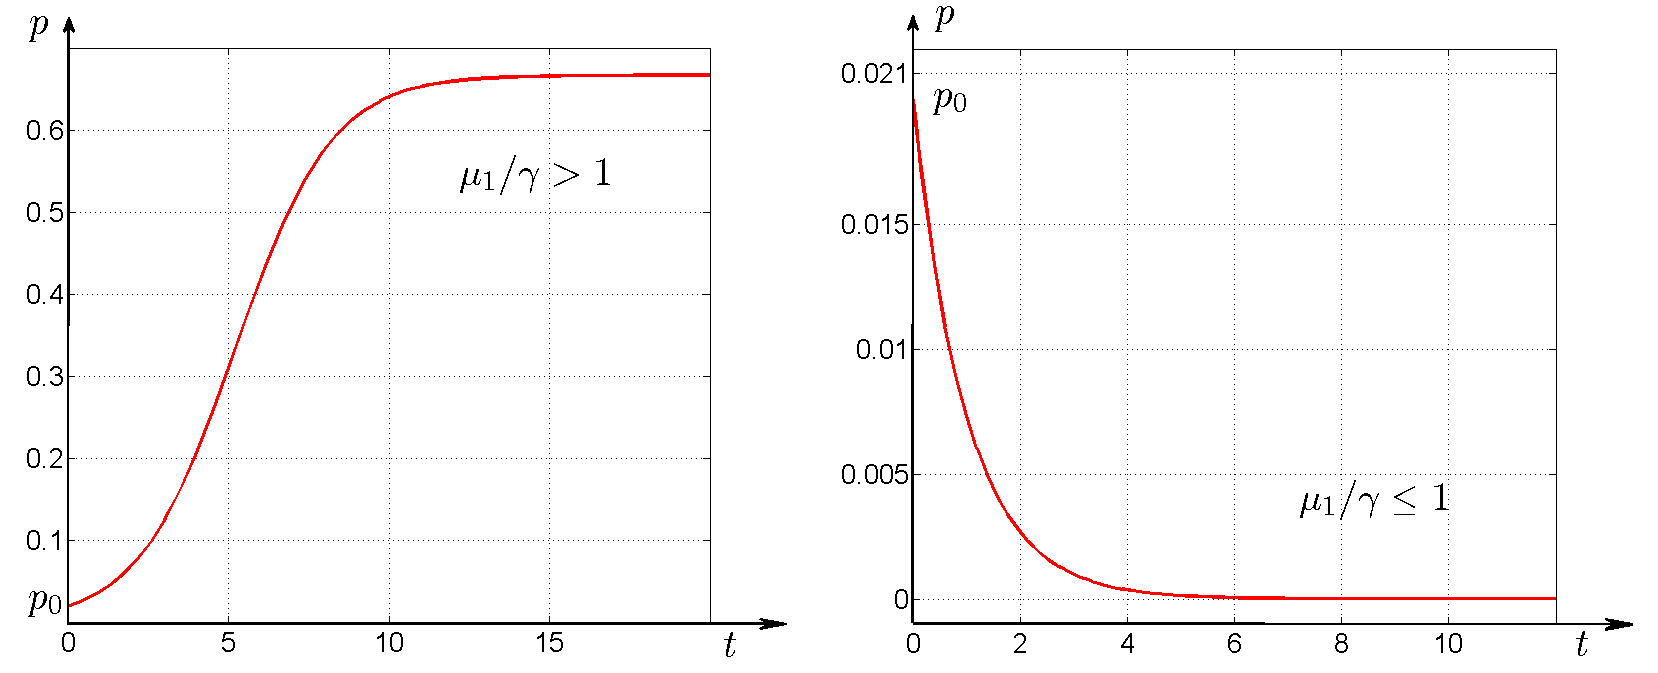
\includegraphics[width=15cm,height=6cm]{5.png}
	\caption{The proportion of drug users over time} % 标题
	\label{SIS}
\end {figure}

We solve the equation and plot the $p(t)$ function, as shown in Figure \ref{SIS}. We discover in the figure that $\mu_1 / \gamma $ serves a threshold: only when $\mu_1 / \gamma \leq 1$, which indicates the control to the drugs is stronger than the spread of drugs, will the number of drug users gradually decrease to zero. We find that under the effect of policies, the number of drug cases start to decline. By analyzing the results of the drug spread depicted by the equation. we find that after four years, the drug use was effectively controlled. The parameter at this time is $\mu_1 / \gamma = 0.5$, indicating that the number of drugs controlled is twice the number of opioid spread.

Under the control of policies, opioid transmissions between the five states as well as the number of opioid cases begin to decrease, and the transition matrix is reduced, as shown in Figure \ref{trans_adjust}. The blue line indicates the number of opioid cases without government's interventions, while the red line indicates the number of opioid cases with certain policies imposed by the government to control the opioid spread. We interpret the results as follows:
\begin {figure}[h]
	\centering % 居中显示
	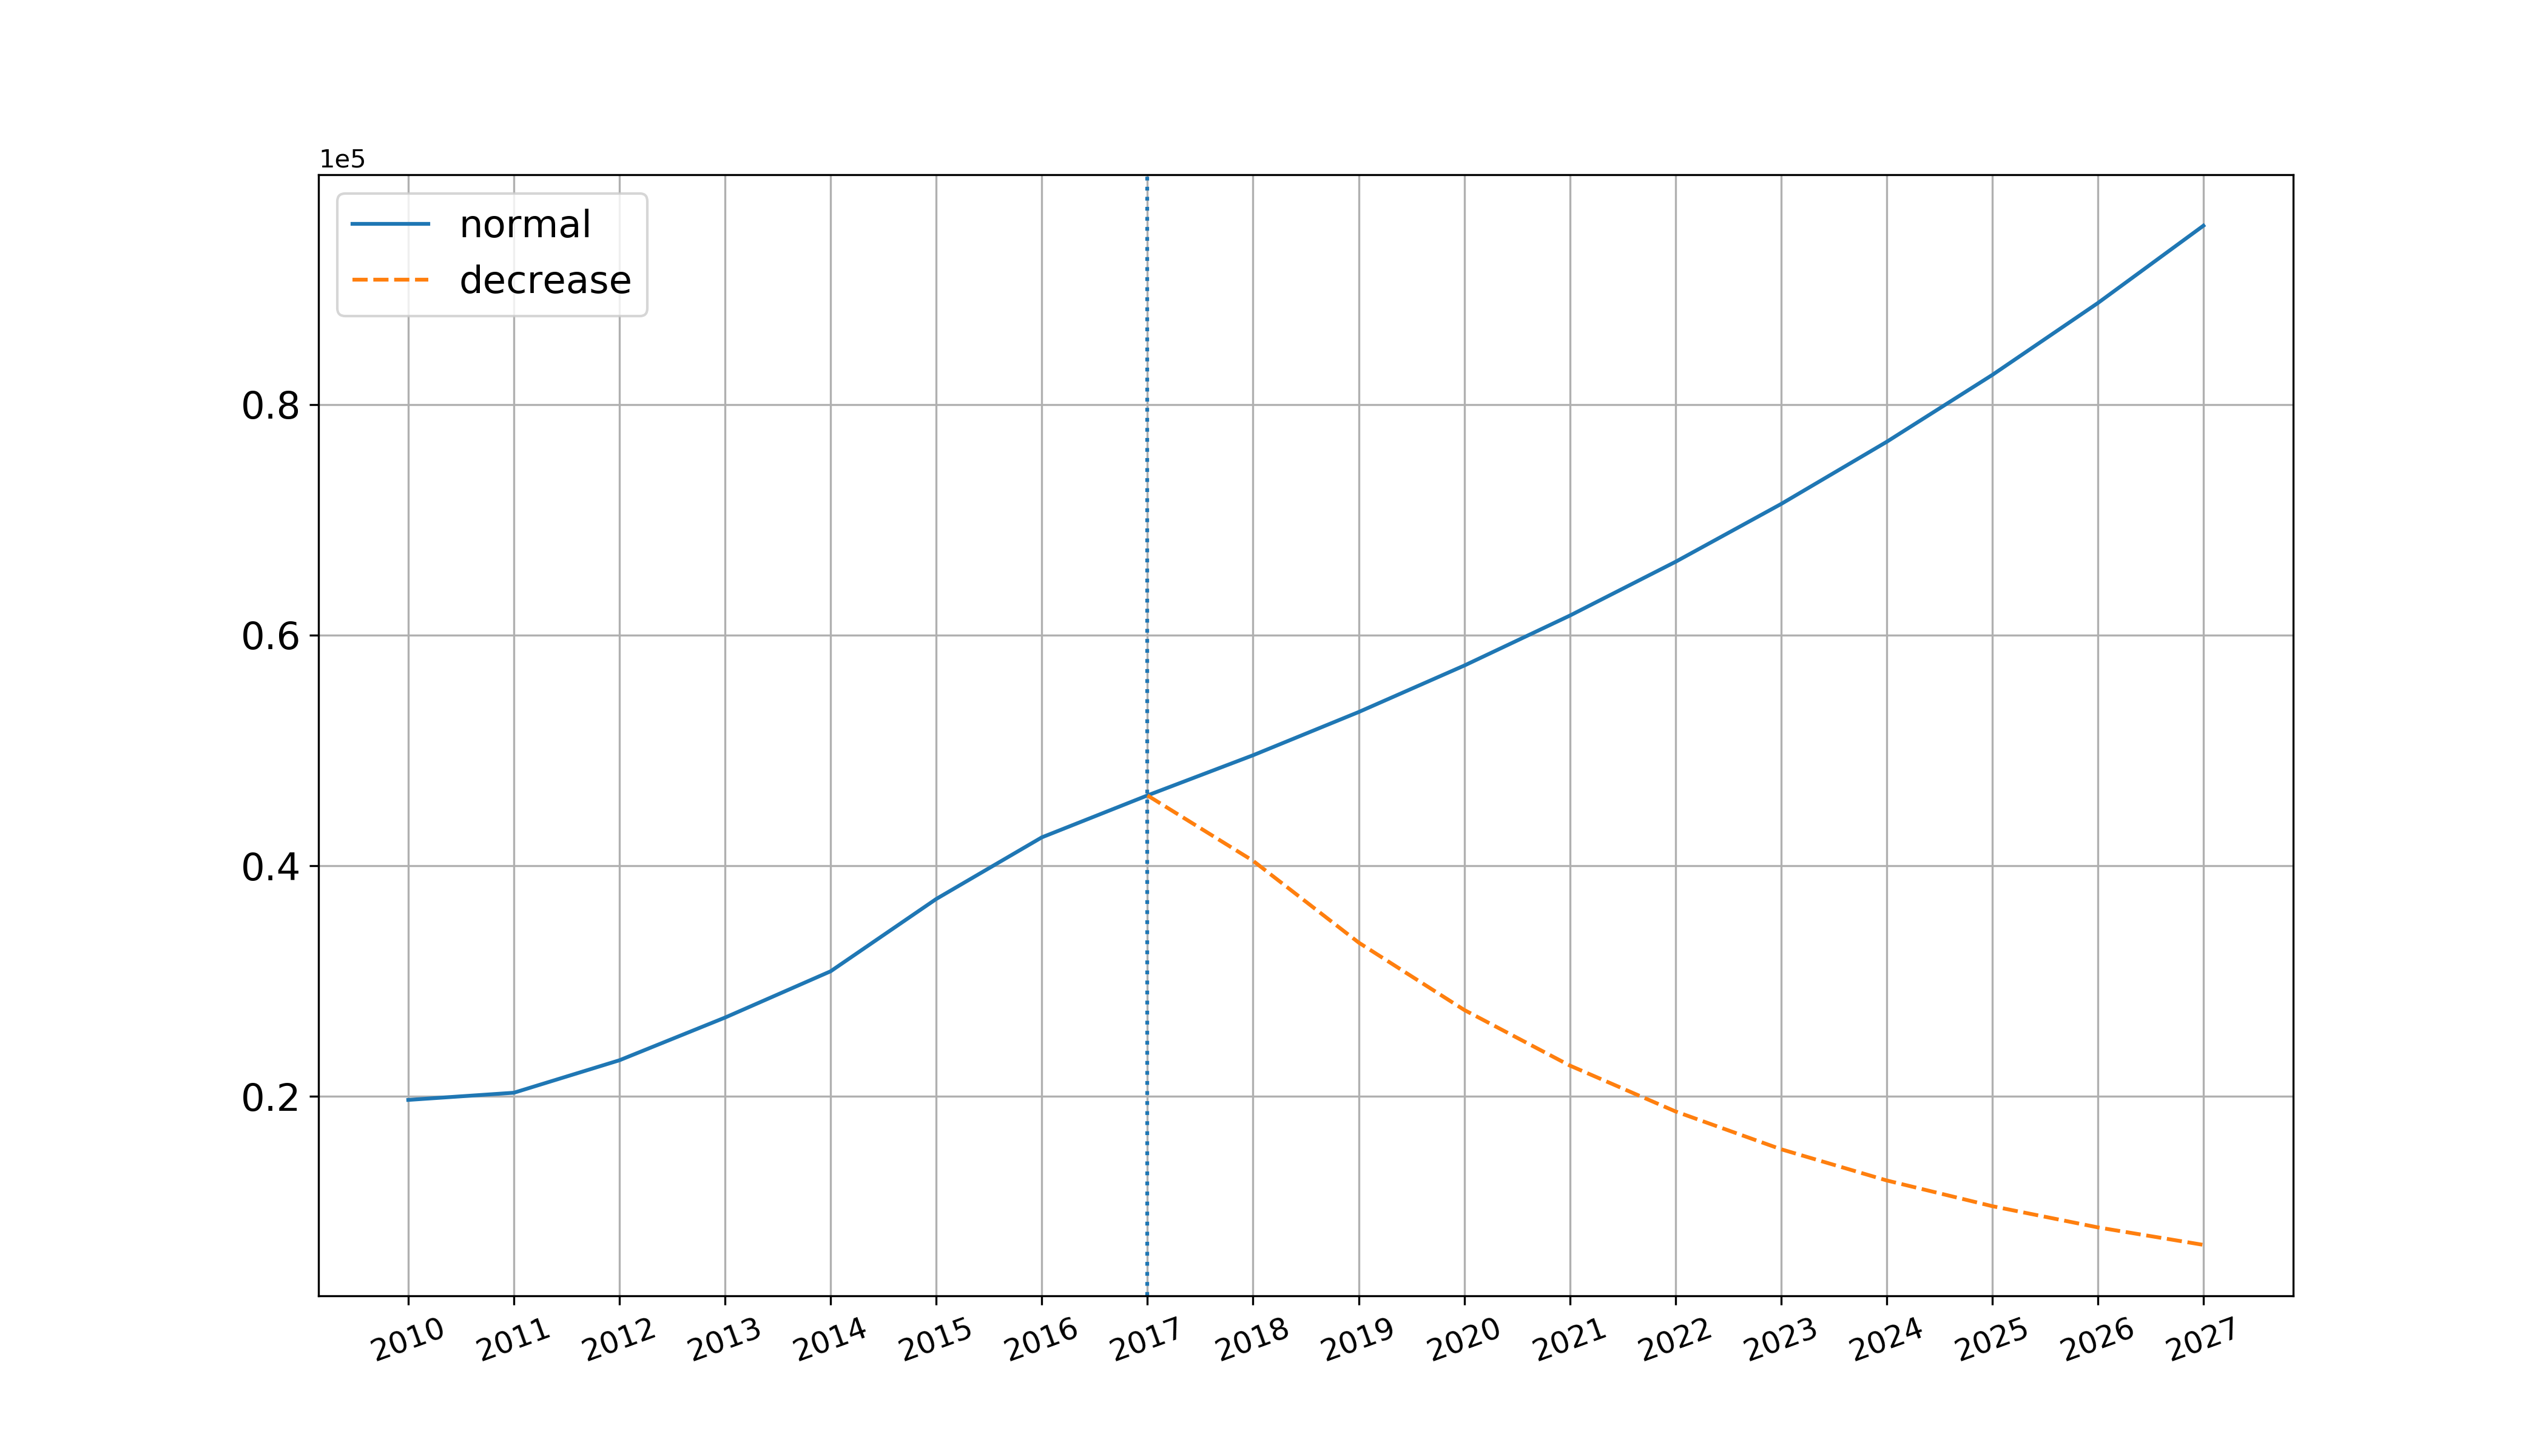
\includegraphics[width=16cm,height=8cm]{6.png}
	\caption{Comparison of number of drug cases} % 标题
	\label{trans_adjust}
\end {figure}

The figure shows that the number of drug cases transmission will gradually decrease, and after 9 years, it will be basically the same as in 2010. The average transition matrix $T$ in 2017-2027 is shown in Table \ref{compare}. Comparing to Table \ref{trans}, the number of opioid cases in Ohio is found to have the most significant reduction, so the supervision in Ohio needs to be strengthened. The overall outflows of the states have been reduced. We sum across the transition matrix, and get the amount of drug transmission to be 2.603 after policies are imposed, where it was 3.543 in 2010-2017. Therefore, the number of opioid cases in the five states is reduced by 26.5\%.

\begin{table}
	\centering
	\caption{Transition matrix for states}
	\vspace{10pt}
	\begin{tabular}{>{\centering\arraybackslash}p{4em}>{\centering\arraybackslash}p{3em}>{\centering\arraybackslash}p{3em}>{\centering\arraybackslash}p{3em}>{\centering\arraybackslash}p{3em}>{\centering\arraybackslash}p{3em}}
		\toprule
		{State}& KY & OH & PA & VA & WV\\\midrule
		KY & 0.027 & 0.129 & 0.070 & 0.036 & 0.003 \\ 
		OH & 0.136 & 0.469 & 0.354 & 0.179 & 0.014 \\ 
		PA & 0.082 & 0.389 & 0.212 & 0.107 & 0.008 \\ 
		VA & 0.035 & 0.167 & 0.091 & 0.047 & 0.004 \\ 
		WV & 0.005 & 0.022 & 0.012 & 0.006 & 0.002 \\ \bottomrule
	\end{tabular}
	\label{compare}
\end{table}

\textbf{\section{Strengths and Weaknesses}}
Based on the modeling process, we make some comments on our model as listed below.
\textbf{\subsection{Strengths}}
\begin{itemize}
	\item We employ transition matrices in our model to analyze the spread and characteristics of opioid use as well as to provide quantitative results for further analysis, which shares a lot of similarities with the Markov chain, leading to a concise, easy-to-understand yet powerful model structure. Our model can also be adapted for other purposes such as computing rankings and analyzing virus transmission, showing good generalizability.
	\item By employing conditional entropy, our model is able to effectively measure the correlations between the opioid cases and socio-economic factors without knowing the concrete relationships (e.g. linear or non-linear) between them.
	\item Two epidemic thresholds are determined for the number and the rate of opioid transmissions, both of which are quantified, making it convenient for government departments to make decisions.
\end{itemize}
\textbf{\subsection{Weaknesses}}
\begin{itemize}
	\item We do not take the opioid spread outside of the five states (KY, OH, PA, VA, WV) into consideration due to the lack of data, which may affect the analysis result.
	\item Although reasonable suggestions are made for the socio-economic factors which shows high correlation with the number of opioid cases, we do not quantify each effect when policies are imposed, instead we represent the effects by a single parameter, the value of which we have provided.
\end{itemize}
\textbf{\section{Sensitivity Analysis}}

The analysis of the spread and flow of drugs is mainly based on the transition matrix $T$. In our assumptions, we assume that the transition matrix does not contain the inflow of opioids from outside the five states, but in actual cases this is not appropriate. We do sensitivity analysis of the transition matrix, in order to prove the robustness of our model.
While imposing strict management inside the state, there may be inflows of opioids from outside the five states, and the inflows may be long-term continuous inflows or indirect outflows. We calculate the transition matrix $T$ in both cases, then do sensitivity analysis of the spread results of the five states. The result is shown in Figure \ref{sensi}.

\begin {figure}[h]
	\centering % 居中显示
	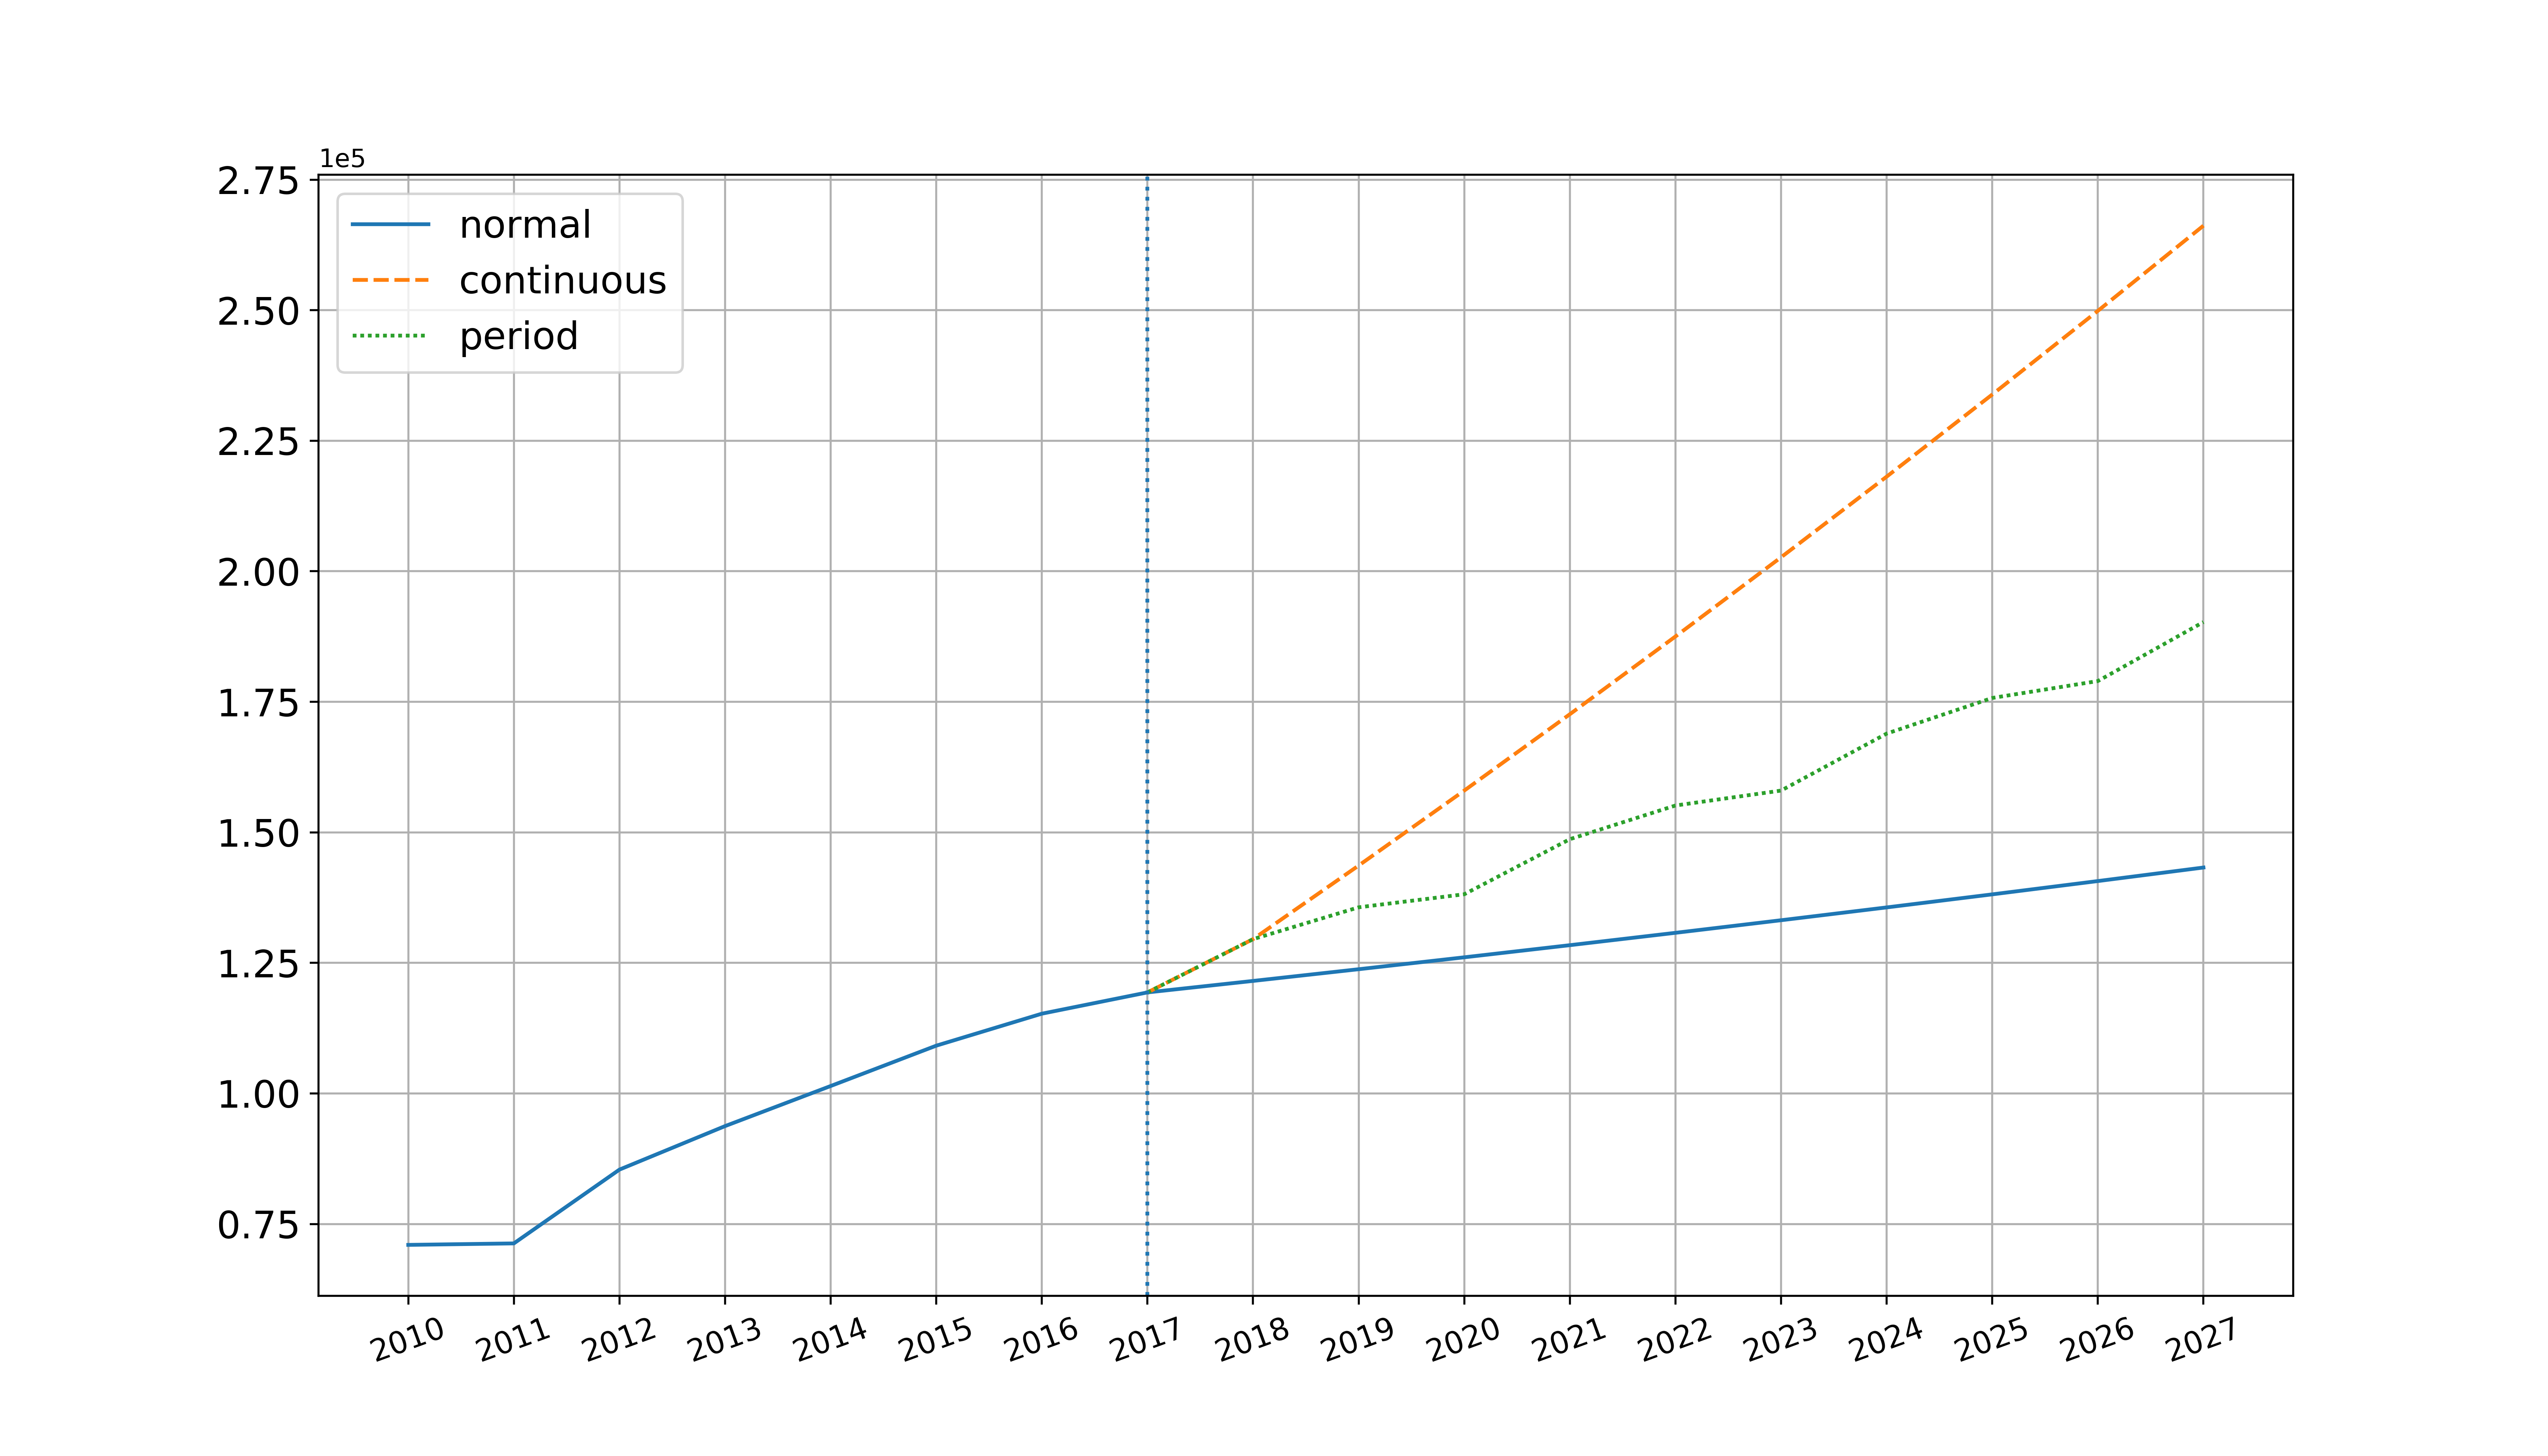
\includegraphics[width=16cm,height=8cm]{7.png}
	\caption{The number of cases} % 标题
	\label{sensi}
\end {figure}
\newpage
Both the continuous and periodical inflows lead to increase in the number of opioids in the state. The result shows that the continuous inflow of opioids has the greatest impact. Although the indirect inflows are incidents, they should also raise the government's concern. In conclusion, the government should not only impose strict regulations on opioids inside the state, but also pay attention to the inflow of opioids from outside the state, and monitors the logistics constantly.
\textbf{\section{Conclusion}}
We build a model to analyze the opioid spread in and between the provided states and counties, determine epidemic thresholds with respect to the number and spread rate of opioid cases, analyze the correlations between the number of opioid cases and various socio-economic factors, then we modify our model to include the most important factors, and provide suggestions to the government based on the factors with high correlations with the number of opioid cases. We also perform simulations to monitor the evolution of opioid use cases in the future. Here are some of our interesting findings:

\begin{itemize}
	\item On a state level, we suggest that Ohio (OH) is the source of opioid use cases. Without policy interventions, there will be even more cases reported in the future.
	\item The epidemic threshold with respect to the spread rate is strongly related to the proportion of drug abuse population and management system of a region, and by setting a lower epidemic threshold, the number of opioid cases in the region can be effectively controlled.
	\item When the government's detection rate of opioid use is higher than the spread rate of opioids, the drug abuse population will be significantly reduced within 2 years. And when the transmission amount of opioid use drops by 26.3\%, the number of opioid cases will decrease to the same level as in 2010.
\end{itemize}

% 因为不输出此部分到目录 \addcontentsline{}{}{}是添加此标题到目录 
\newpage
\textbf{\section*{References}\addcontentsline{toc}{section}{References}}
\fancyhf{}
\fancyhead[R]{ }
\fancyhead[L]{ }
\bibliography{books}
\Large
\bibliographystyle{IEEEtran}

\newpage
\textbf{\section*{Appendices}\addcontentsline{toc}{section}{Appendices for Code and Data}} 
\fontsize{13pt}{12.5pt}\selectfont
Here is Code we used in our model, which python is the main development language.
\vspace{7pt}
\textbf{\subsection*{Appendices A}}
\begin {figure}[h]
	\centering % 居中显示
	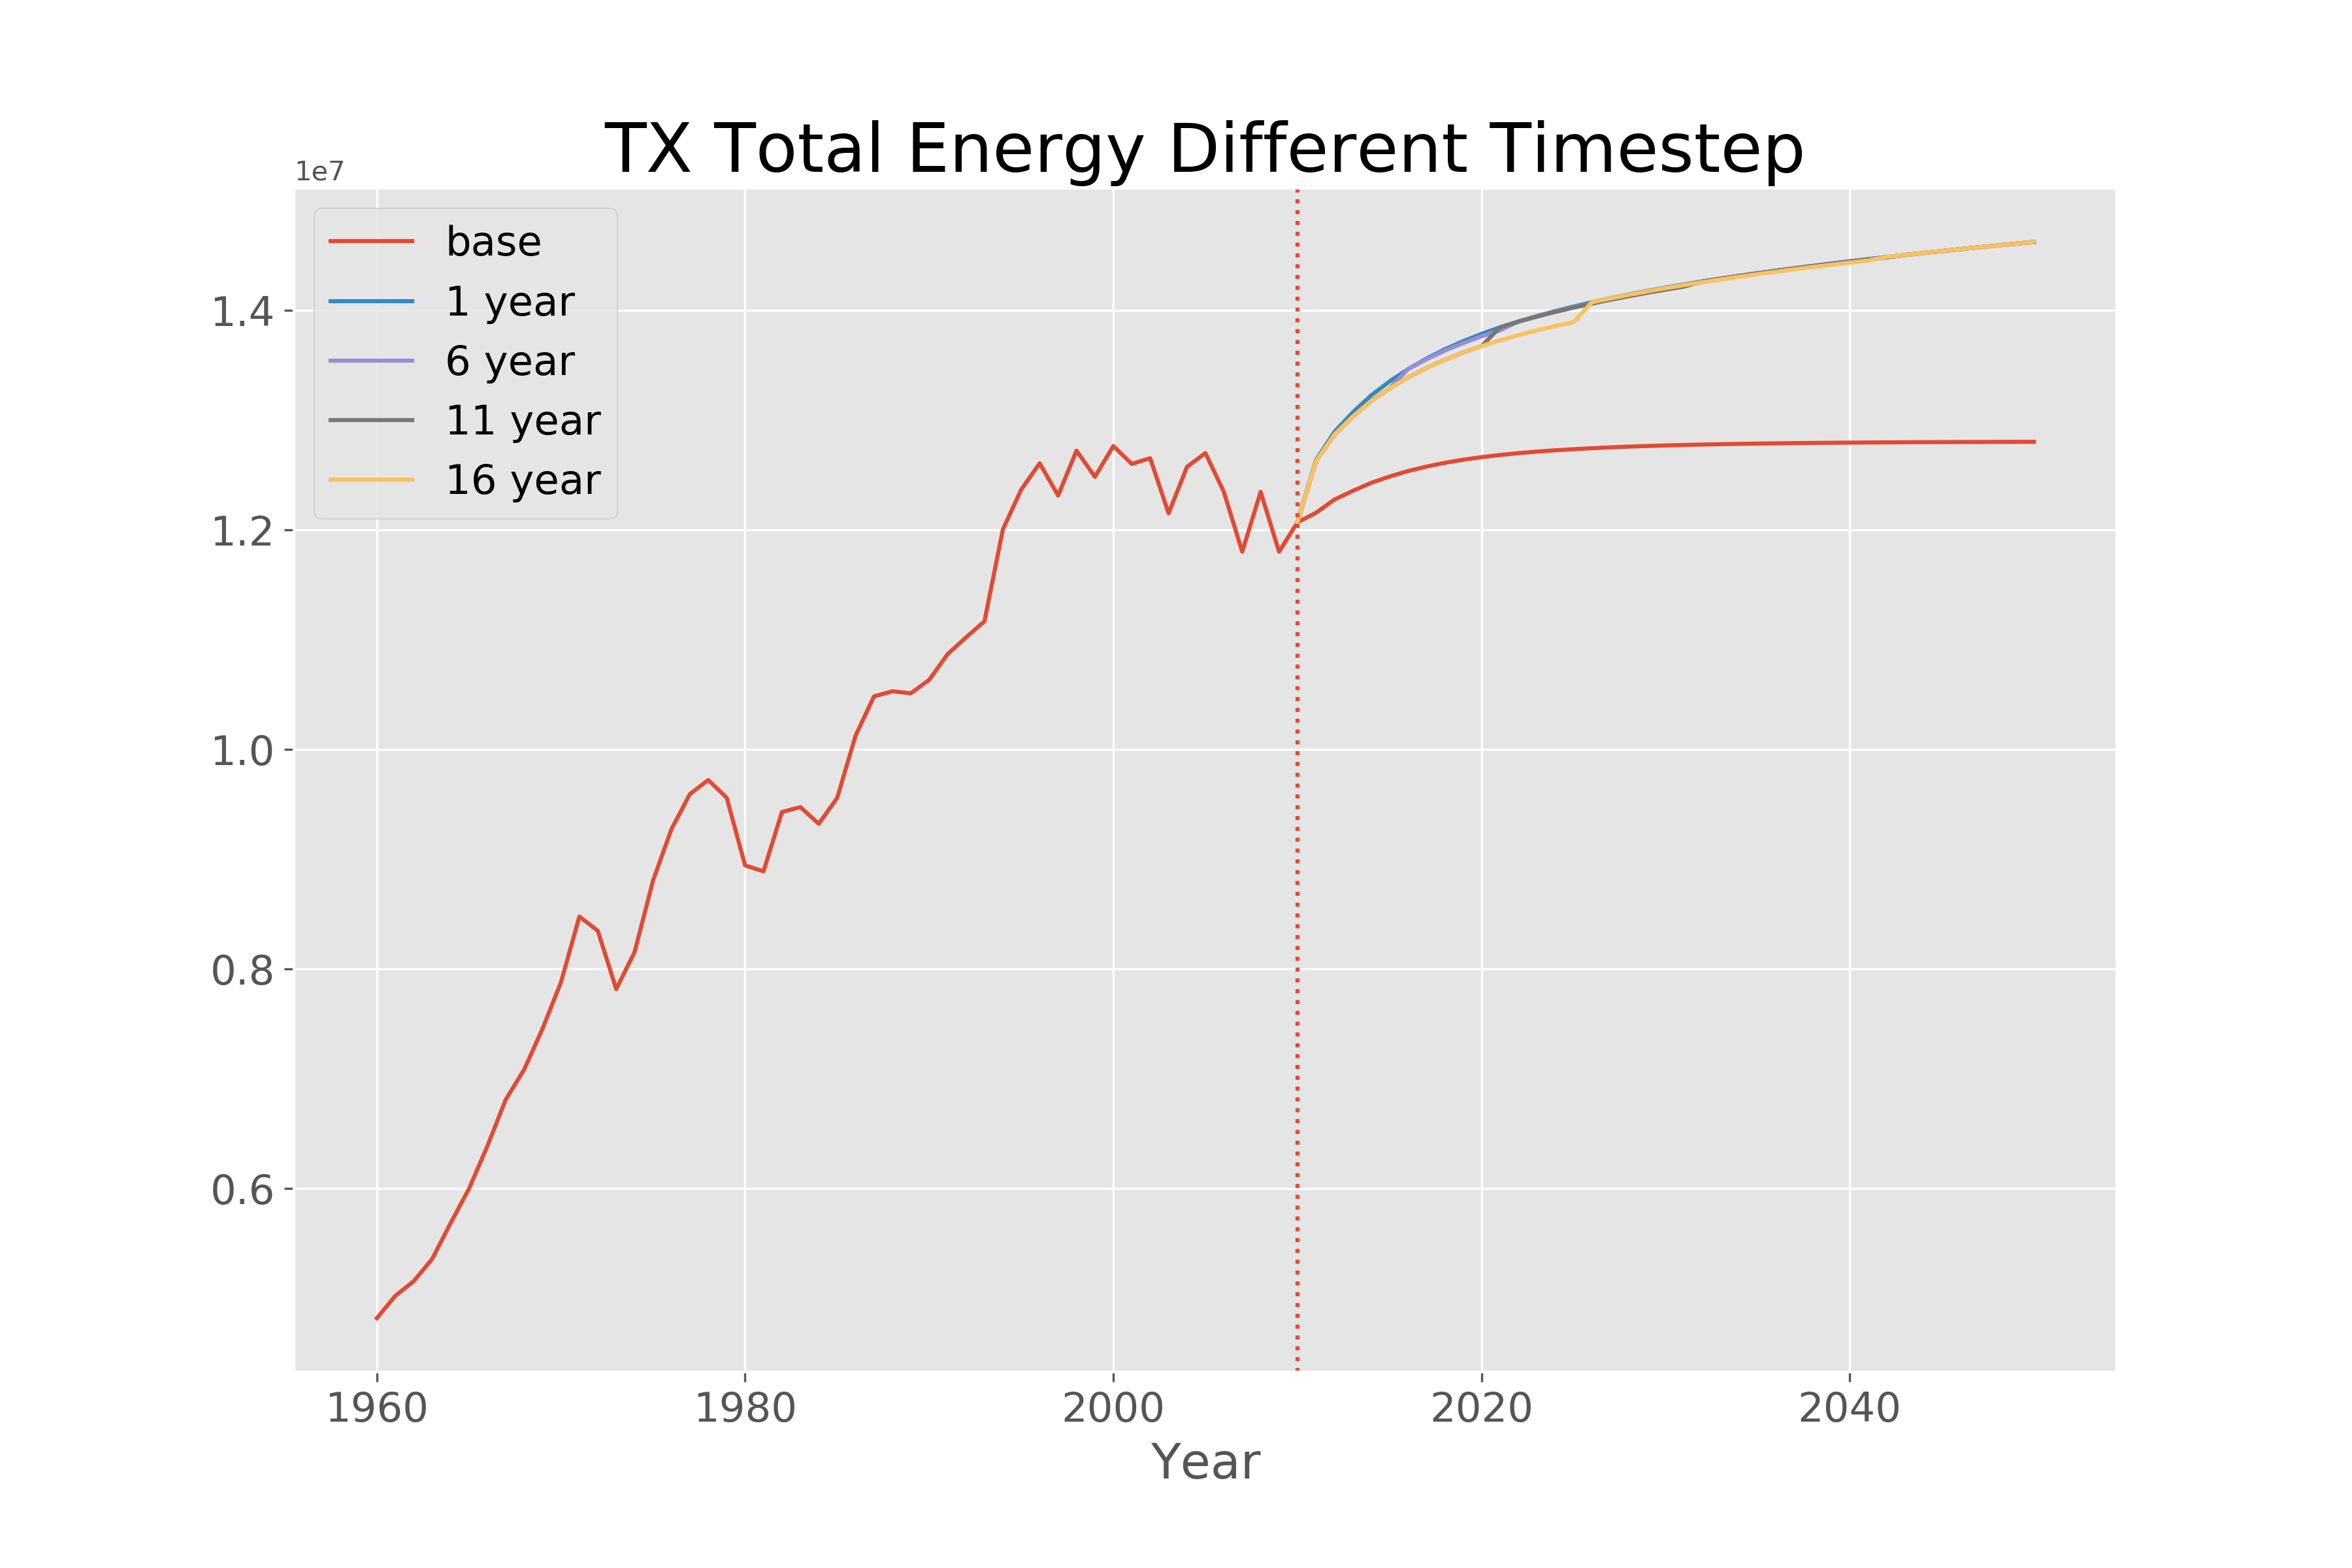
\includegraphics[width=15cm,height=12cm]{8.png}
	\caption{Transition matrix for synthetic opioid spread rate in West Virginia} % 标题
\end {figure}

\textbf{\subsection*{Appendices B: Forecast and Draw the Drugs of 2018-2027 Cases}}
\noindent{\rule{\textwidth}{0.2mm}}
\vspace{-18pt} 
\fontsize{13pt}{12.5pt}\selectfont
{
	\lstinputlisting[language=python]{predict.py}
}
\vspace{-15pt}
\noindent{\rule{\textwidth}{0.2mm}}
\textbf{\subsection*{Appendices C: The Program for Calculating Information Gain}}
\noindent{\rule{\textwidth}{0.2mm}}
\vspace{-18pt} 
\fontsize{13pt}{12.5pt}\selectfont
{
	\lstinputlisting[language=python]{information.py}
}
\vspace{-15pt}
\noindent{\rule{\textwidth}{0.2mm}}
\textbf{\subsection*{Appendices D: Transition Matrix of Five States}}
\noindent{\rule{\textwidth}{0.2mm}}
\vspace{-18pt} 
\fontsize{13pt}{12.5pt}\selectfont
{
	\lstinputlisting[language=python]{states.py}
}
\vspace{-15pt}
\noindent{\rule{\textwidth}{0.2mm}}

\end{document}